%%%%%%%%%%%%%%%%%%%%%%%%%%%%%%%%%%%%%%%%%%%%%%%%%%%%%%%%%%%%%%%%%%%%%%%%%%%
%% This file is part of the book
%%
%% Algorithmic Graph Theory
%% http://code.google.com/p/graph-theory-algorithms-book/
%%
%% Copyright (C) 2009, 2010 Minh Van Nguyen <nguyenminh2@gmail.com>
%%
%% See the file COPYING for copying conditions.
%%%%%%%%%%%%%%%%%%%%%%%%%%%%%%%%%%%%%%%%%%%%%%%%%%%%%%%%%%%%%%%%%%%%%%%%%%%

%% simple graph
\subfigure[Simple graph.]{
\label{fig:introduction:triangle_simple_graph}
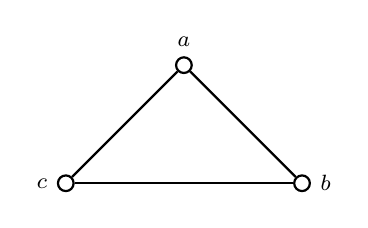
\begin{tikzpicture}
[lineDecorate/.style={-,thick},%
  nodeDecorate/.style={shape=circle,inner sep=2pt,draw,thick}]
%% nodes or vertices
\foreach \nodename/\x/\y/\direction/\navigate in {
  c/-1.5/0/left/west, b/1.5/0/right/east, a/0/1.5/above/north}
{
  \node (\nodename) at (\x,\y) [nodeDecorate] {};
  \node [\direction] at (\nodename.\navigate) {\footnotesize$\nodename$};
}
%% edges or lines
\path
\foreach \startnode/\endnode in {a/b, b/c, c/a}
{
  (\startnode) edge[lineDecorate] node {} (\endnode)
};
\end{tikzpicture}
}
\quad
%%
%%
%% digraph
\subfigure[Digraph.]{
\label{fig:introduction:triangle_digraph}
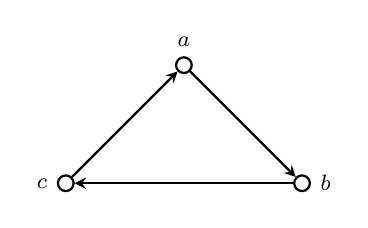
\begin{tikzpicture}
[arrowDecorate/.style={->,>=stealth,thick},%
  nodeDecorate/.style={shape=circle,inner sep=2pt,draw,thick}]
%% nodes or vertices
\foreach \nodename/\x/\y/\direction/\navigate in {
  c/-1.5/0/left/west, b/1.5/0/right/east, a/0/1.5/above/north}
{
  \node (\nodename) at (\x,\y) [nodeDecorate] {};
  \node [\direction] at (\nodename.\navigate) {\footnotesize$\nodename$};
}
%% edges or lines
\path
\foreach \startnode/\endnode in {a/b, b/c, c/a}
{
  (\startnode) edge[arrowDecorate] node {} (\endnode)
};
\end{tikzpicture}
}
\quad
%%
%%
%% multidigraph
\subfigure[Multidigraph.]{
\label{fig:introduction:Konigsberg_multidigraph}
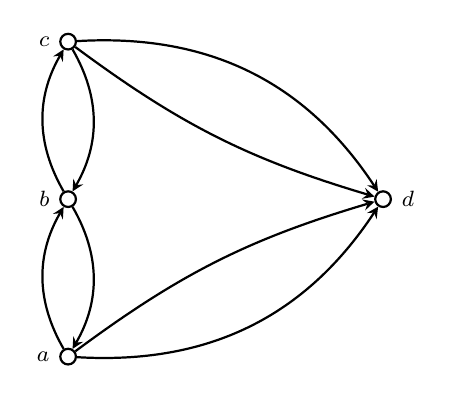
\begin{tikzpicture}
[arrowDecorate/.style={->,>=stealth,thick},%
  nodeDecorate/.style={shape=circle,inner sep=2pt,draw,thick}]
%% nodes or vertices
\foreach \nodename/\x/\y/\direction/\navigate in {
  a/0/0/left/west, b/0/2/left/west, c/0/4/left/west, d/4/2/right/east}
{
  \node (\nodename) at (\x,\y) [nodeDecorate] {};
  \node [\direction] at (\nodename.\navigate) {\footnotesize$\nodename$};
}
%% edges or lines
\path
\foreach \startnode/\endnode/\bend in {
  a/b/bend left, a/d/bend right, b/c/bend left, c/b/bend left,
  b/a/bend left, c/d/bend left}
{
  (\startnode) edge[arrowDecorate,\bend] node {} (\endnode)
}
%% multiple directed edges
(a) edge[arrowDecorate,bend left=10] node {} (d)
(c) edge[arrowDecorate,bend right=10] node {} (d);
\end{tikzpicture}
}
